\documentclass[11pt,a4paper]{article}

\usepackage{gastex}
\usepackage{etoolbox}
% \newcommand{\showLoesung}{2} %<---als Schalter
% \newcommand{\showInhalt}{1} %<---als Schalter
% \newcommand{\volbert}{3} %<---als Schalter

\usepackage{alltt,moreverb,amsmath,enumerate}
\usepackage[normalem]{ulem}
\usepackage[T1]{fontenc}
\usepackage{ae,aecompl} %helvet,mathptm
%\usepackage[left=15mm,right=15mm,top=20mm,bottom=20mm]{geometry}
\usepackage[margin=.5in]{geometry}
%\usepackage[latin1]{inputenc} % f�r Linux
\usepackage[utf8]{inputenc} % Umlaute etc. direkt schreiben (unter Windows)
\usepackage[german]{babel}
\usepackage[url]{oth-logoPNG}
%\usepackage{i2sym,i2ams}

\usepackage{tikz}
\usetikzlibrary{arrows,shapes,trees,positioning,automata,decorations.pathreplacing,decorations.pathmorphing}
\usepackage{tkz-graph}
\usepackage{color}

\usepackage{longtable}
\usepackage{tabularx}

%\usepackage{epic}
%\usepackage{eepic}
\usepackage{comment,ifthen}
\usepackage{../include/todo}

\usepackage[T1]{fontenc}
\usepackage{textcomp}

\usepackage{listings}                   % Listings in Core-Erlang und Maude
\usepackage{lstmisc}

\usepackage{epic}                       % Bildbefehle (picture)
%\usepackage{eepic}                      % erweiterte Bildbefehle

\usepackage{bbm}                        % Mengensymbole (N,C,R,B)
\usepackage{latexsym}                   % zusaetzliche Mathesymbole
\usepackage{amsmath}                    % Mathepaket von der AMS
\usepackage{amstext}
\usepackage{amsfonts}
\usepackage{stmaryrd}                   % zusaetzliche Mathesymbole
\usepackage{mathtools}
\usepackage{amsthm}
\usepackage{cancel}

\usepackage{hyperref}
\usepackage{url}                        % Zum Setzen von URLs in typewriter-face

\pagestyle{empty}

\let\epsilon=\varepsilon
\let\phi=\varphi

\frenchspacing

\setlength{\parindent}{0pt}
\setlength{\textwidth}{18.6cm}
\setlength{\textheight}{26.5cm}
\setlength{\hfuzz}{1mm}

%%% Read dates of assignments from file
\usepackage{xparse}
\ExplSyntaxOn
\ior_new:N \g_hringriin_file_stream

\NewDocumentCommand{\ReadFile}{mm}
 {
  \hringriin_read_file:nn { #1 } { #2 }
  \cs_new:Npn #1 ##1
   {
    \str_if_eq:nnTF { ##1 } { * }
      { \seq_count:c { g_hringriin_file_ \cs_to_str:N #1 _seq } }
      { \seq_item:cn { g_hringriin_file_ \cs_to_str:N #1 _seq } { ##1 } }
   }
 }

\cs_new_protected:Nn \hringriin_read_file:nn
 {
  \ior_open:Nn \g_hringriin_file_stream { #2 }
  \seq_gclear_new:c { g_hringriin_file_ \cs_to_str:N #1 _seq }
  \ior_map_inline:Nn \g_hringriin_file_stream
   {
    \seq_gput_right:cx 
     { g_hringriin_file_ \cs_to_str:N #1 _seq }
     { \tl_trim_spaces:n { ##1 } }
   }
  \ior_close:N \g_hringriin_file_stream
 }

\ExplSyntaxOff

\ReadFile{\uebungsabgabe}{../skel/UEBUNGSABGABE.def}

%%% Read subject info from file
\newcommand{\dozent}[1]{\def\DOZENT{#1}}
\newcommand{\tutoren}[1]{\def\TUTOREN{#1}}
\newcommand{\vorlesung}[1]{\def\VORLESUNG{#1}}
\newcommand{\semester}[1]{\def\SEMESTER{#1}}

\InputIfFileExists{../skel/VORLESUNG.def}{\providecommand{\TUTOREN}{}}%
{\typeout{***********}
 \typeout{Warnung: Kein File vorhanden, das die Vorlesung spezifiziert!}
 \typeout{Spezifikation muss daher im Text des Blattes oder ueber die
          Tastatur erfolgen.}
 \typeout{***********}}

\def\Uebung#1#2#3{
  \othLehrstuhlLogo[\DOZENT]
  \begin{center}
	{~\\[-2em]\Large\bf \VORLESUNG}\\[0.5em]
    \LARGE --~Tutorium #1 (Übung #2)~--\\[4mm]
  \
  \normalsize
  \textbf{#3}
    \rule{\textwidth}{0.1pt}\\[1cm]
  \end{center}
}

\def\Hinweis#1{
	{~\\[-3em]\bf Hinweis: }
	\begin{minipage}[t]{16.5cm}
	#1
	\end{minipage}\\[1em]
    \rule{\textwidth}{0.1pt}
}

\def\Tipps#1{
	{~\\[-3em]\bf Tipps: }
	\begin{minipage}[t]{16.5cm}
	#1
	\end{minipage}\\[1em]
    \rule{\textwidth}{0.1pt}
}
  
\def\MyHeader{
  \othLehrstuhlLogo[Prof.~Dr.~rer.~nat.~Carsten~Kern]%[Carsten~Kern,~Stefan~Rieger]
}

\newcommand{\sem}[1]{[\![#1\,]\!]}

\def\aufgabe#1#2{\subsection*{Aufgabe #1 (#2)}\par}
\def\endaufgabe{}

\newenvironment{loesung}{\subsection*{L\"osungsvorschlag:}}{}
\newenvironment{hinweis}{}{}
\ifthenelse{\isundefined{\showLoesung}}{\excludecomment{loesung}}{\pagestyle{plain}\excludecomment{hinweis}}

\newenvironment{tipps}{}{}
\ifthenelse{\isundefined{\showTipps}}{\excludecomment{tipps}}{\excludecomment{hinweis}}

\newenvironment{inhalt}{\subsection*{Kommentar:}}{}
\ifthenelse{\isundefined{\showInhalt}}{\excludecomment{inhalt}}{}

\long\def\Exercise#1#2{\begin{exercise}{#1}#2\end{exercise}}

\def\underbar#1{%
  \setbox0=\hbox{#1}%
  \dimen0=\dp0\relax%
  \dp0=0pt%
  \setbox0=\hbox{\underline{\box0}}%
  \dp0=\dimen0\relax%
  \box0%
  }

\makeatletter
\def\@makeunderbar[#1]#2{\expandafter\def\csname#1\endcsname{\underbar{#2}}}
\def\makeunderbar{\@ifnextchar[{\@makeunderbar}{\@makeunderbar[]}}
\makeatother

\def\T{\mathrm{T}}
\def\P{\mathrm{P}}
\def\CT{\mathrm{CT}}
\def\COp{\mathrm{COp}}

\makeunderbar{Comp}
\makeunderbar{Ops}
\makeunderbar{trans}
\makeunderbar[strans]{s-trans}
\makeunderbar[ntrans]{n-trans}
\makeunderbar{fix}

\def\labelenumi{\alph{enumi})}
\let\<=\langle
\let\>=\rangle

\parindent=0pt
\parskip=1ex

\definecolor{javared}{rgb}{0.6,0,0} % for strings
\definecolor{javagreen}{rgb}{0.25,0.5,0.35} % comments
\definecolor{javapurple}{rgb}{0.5,0,0.35} % keywords
\definecolor{javadocblue}{rgb}{0.25,0.35,0.75} % javadoc
 
\lstset{language=C++,
basicstyle=\ttfamily\footnotesize,
keywordstyle=\color{javapurple}\bf,
stringstyle=\color{javared},
commentstyle=\color{javagreen}\it\bf,
morecomment=[s][\color{javadocblue}]{/**}{*/},
numbers=left,
numberstyle=\tiny\color{gray},
stepnumber=1,
numbersep=10pt,
tabsize=3,
showspaces=false,
showstringspaces=false}

\usepackage{enumitem}
\usepackage{algpseudocode}
\usepackage{caption}
\usepackage{subcaption}
\usepackage{placeins}
\usepackage{multicol}
\usepackage{slashbox}
\usepackage{fancyvrb}
\usepackage{ulem}
\usepackage{amssymb}

\begin{document}
\thispagestyle{empty}
\DeclareRobustCommand{\ttfamily}{\fontencoding{T1}\fontfamily{lmtt}\selectfont}

\newcommand{\quotes}[1]{\glqq{}#1\grqq{}}

\SpecialUebung{13}{Wiederholung}{Simon Thelen}{20. Januar 2021}  % FIXME: Blattnummer, Datum, Zeit

%%%%%%%%%%%%%%%%%%%%%%%%%%%%%%%%%%%%%%%%%%%%%%%%%%%%%%%%%%%%%%%%%%%%%%

\ifcsdef{showLoesung}{
\textbf{Bitte beachten Sie:} Die Lösungen können trotz sorgfältiger Prüfung Fehler enthalten.
Bei Fragen oder Unklarheiten kontaktieren Sie bitte den Tutor oder Dozenten in Tutorien, Übungen oder nach Vorlesungen.
}{}

\begin{aufgabe}{1}{Verständnisfragen}
    Sind folgende Aussagen \emph{richtig} oder \emph{falsch}?
    \begin{enumerate}
        \item $\log(n!) = \Theta(n \log n)$
        \item Selection Sort ist stabil
        \item Mergesort hat Laufzeit $\Omega(n \log n)$
        \item Beim Löschen eines Elements aus einem AVL-Baum ist maximal eine (Doppelt)Rotation nötig.
        \item Es ist erlaubt, dass die Wurzel eines B-Baumes der Ordnung 5 nur ein Element enthält.
        \item $h(s, i) = (s + i \cdot h'(s)) \bmod 13$ mit $h'(s) = s \bmod 7$ ist eine geeignete Funktion für Hashing mit offener Adressierung.
        \item Zum Lösen des APSP-Problems hat der Floyd-Warshall-Algorithmus für alle Eingaben eine bessere Laufzeit als Dijkstra von jedem Knoten aus zu starten.
    \end{enumerate}
    Nur für den Kurs von Herrn Kern:
    \begin{enumerate}
        \setcounter{enumi}{7}
        \item Die Laufzeit von $\mathrm{NL}^*$ ist für die gleiche Sprache stets höher als die von $\mathrm{L}^*$.
        \item Die Tabellenzeile $-+-$ ist bei $\mathrm{NL}^*$ immer prim.
    \end{enumerate}
    Nur für den Kurs von Herrn Volbert:
    \begin{enumerate}
        \setcounter{enumi}{7}
        \item Aus $L \leq_p \mathrm{SAT}$ folgt: $L$ ist NP-vollständig.
        \item Aus $\mathrm{SAT} \leq_p L$ folgt: $L$ ist NP-vollständig.
    \end{enumerate}
\end{aufgabe}

\begin{aufgabe}{2}{$O$-Kalkül}
    Zeigen oder widerlegen Sie folgende Aussagen:
    \begin{enumerate}
        \item $3^{2n} = O(3^n)$
        \item $\log_3(2n) = \Omega(\log n)$
        % \item $5^{\log(n)} \in \Omega(n^2)$
        \item $\sum\limits_{i=0}^n \frac{i + 2^i}{2} = \Omega(2^n)$
    \end{enumerate}
\end{aufgabe}
\begin{aufgabe}{3}{Rekursionsgleichungen}
    \begin{enumerate}
        \item Lösen Sie die Rekursionsgleichung $T(1) = 1, \,\, T(n) = 2T(n / 4) + \sqrt{n}$ mithilfe des Master-Theorems.
        \item Lösen Sie die Rekursionsgleichung $T(1) = 1, \,\, T(n) = 4T(n / 2) + n^2$ mithilfe des Iterationsmethode.
%         \item Gegeben sei folgender Algorithmus:
%         \begin{lstlisting}[language=c++]
% int algorithm(int a[], int n) {
%     int sum = 0;
%     for (int i = 0; i < n; i++) sum += a[i];
%     if (n <= 2) return sum;
%     return sum + algorithm(a, 2/3 * n) * 2;
% }
%         \end{lstlisting}
        Geben Sie die Worst-Case-Laufzeit des Algorithmus als Rekursionsgleichung an und lösen Sie die Gleichung mithilfe des Master-Theorems.
    \end{enumerate}
\end{aufgabe}
\begin{aufgabe}{4}{Vollständige Induktion}
    Gegeben sei die Folge der Fibonacci-Zahlen: $f(1) = 1$, $f(2) = 1$ und $f(n) = f(n - 1) + f(n - 2)$ für alle $n > 2$.
    Zeigen Sie mittels vollständiger Induktion, dass $f(n) \leq 2^{n - 1}$ für alle $n \in \mathbb{N}$.
\end{aufgabe}
\begin{aufgabe}{5}{Sortieralgorithmen}
    \begin{enumerate}
        \item Sie möchten folgendes Array mittels Quicksort sortieren: $(3, 4, 1, 5, 2, 6)$.
        Geben Sie die Reihenfolge der Elemente nach dem ersten Aufruf von \texttt{preparePartition} an.
        Wie oft wird die Funktion \texttt{quickSort(arr, start, end)} insgesamt aufgerufen?
        \item Sie möchten folgendes Array mittels Heapsort sortieren: $(1, 5, 3, 6, 2, 4)$.
        Stellen die Heap-Eigenschaft im Array mittels \texttt{buildMaxHeap} her.
        Löschen Sie anschließend mittels \texttt{extractMax} die beiden größten Elemente des Heaps.
        Geben Sie die resultierenden Heaps (jeweils nach den drei Operationen) an.
    \end{enumerate}
\end{aufgabe}
\begin{aufgabe}{6}{Suchbäume}
    \begin{enumerate}
        \item Löschen Sie bei folgendem AVL-Baum den markierten Knoten. Geben Sie alle Zwischenschritte und Rotationen an.
        \begin{figure}[h!]
            \centering
            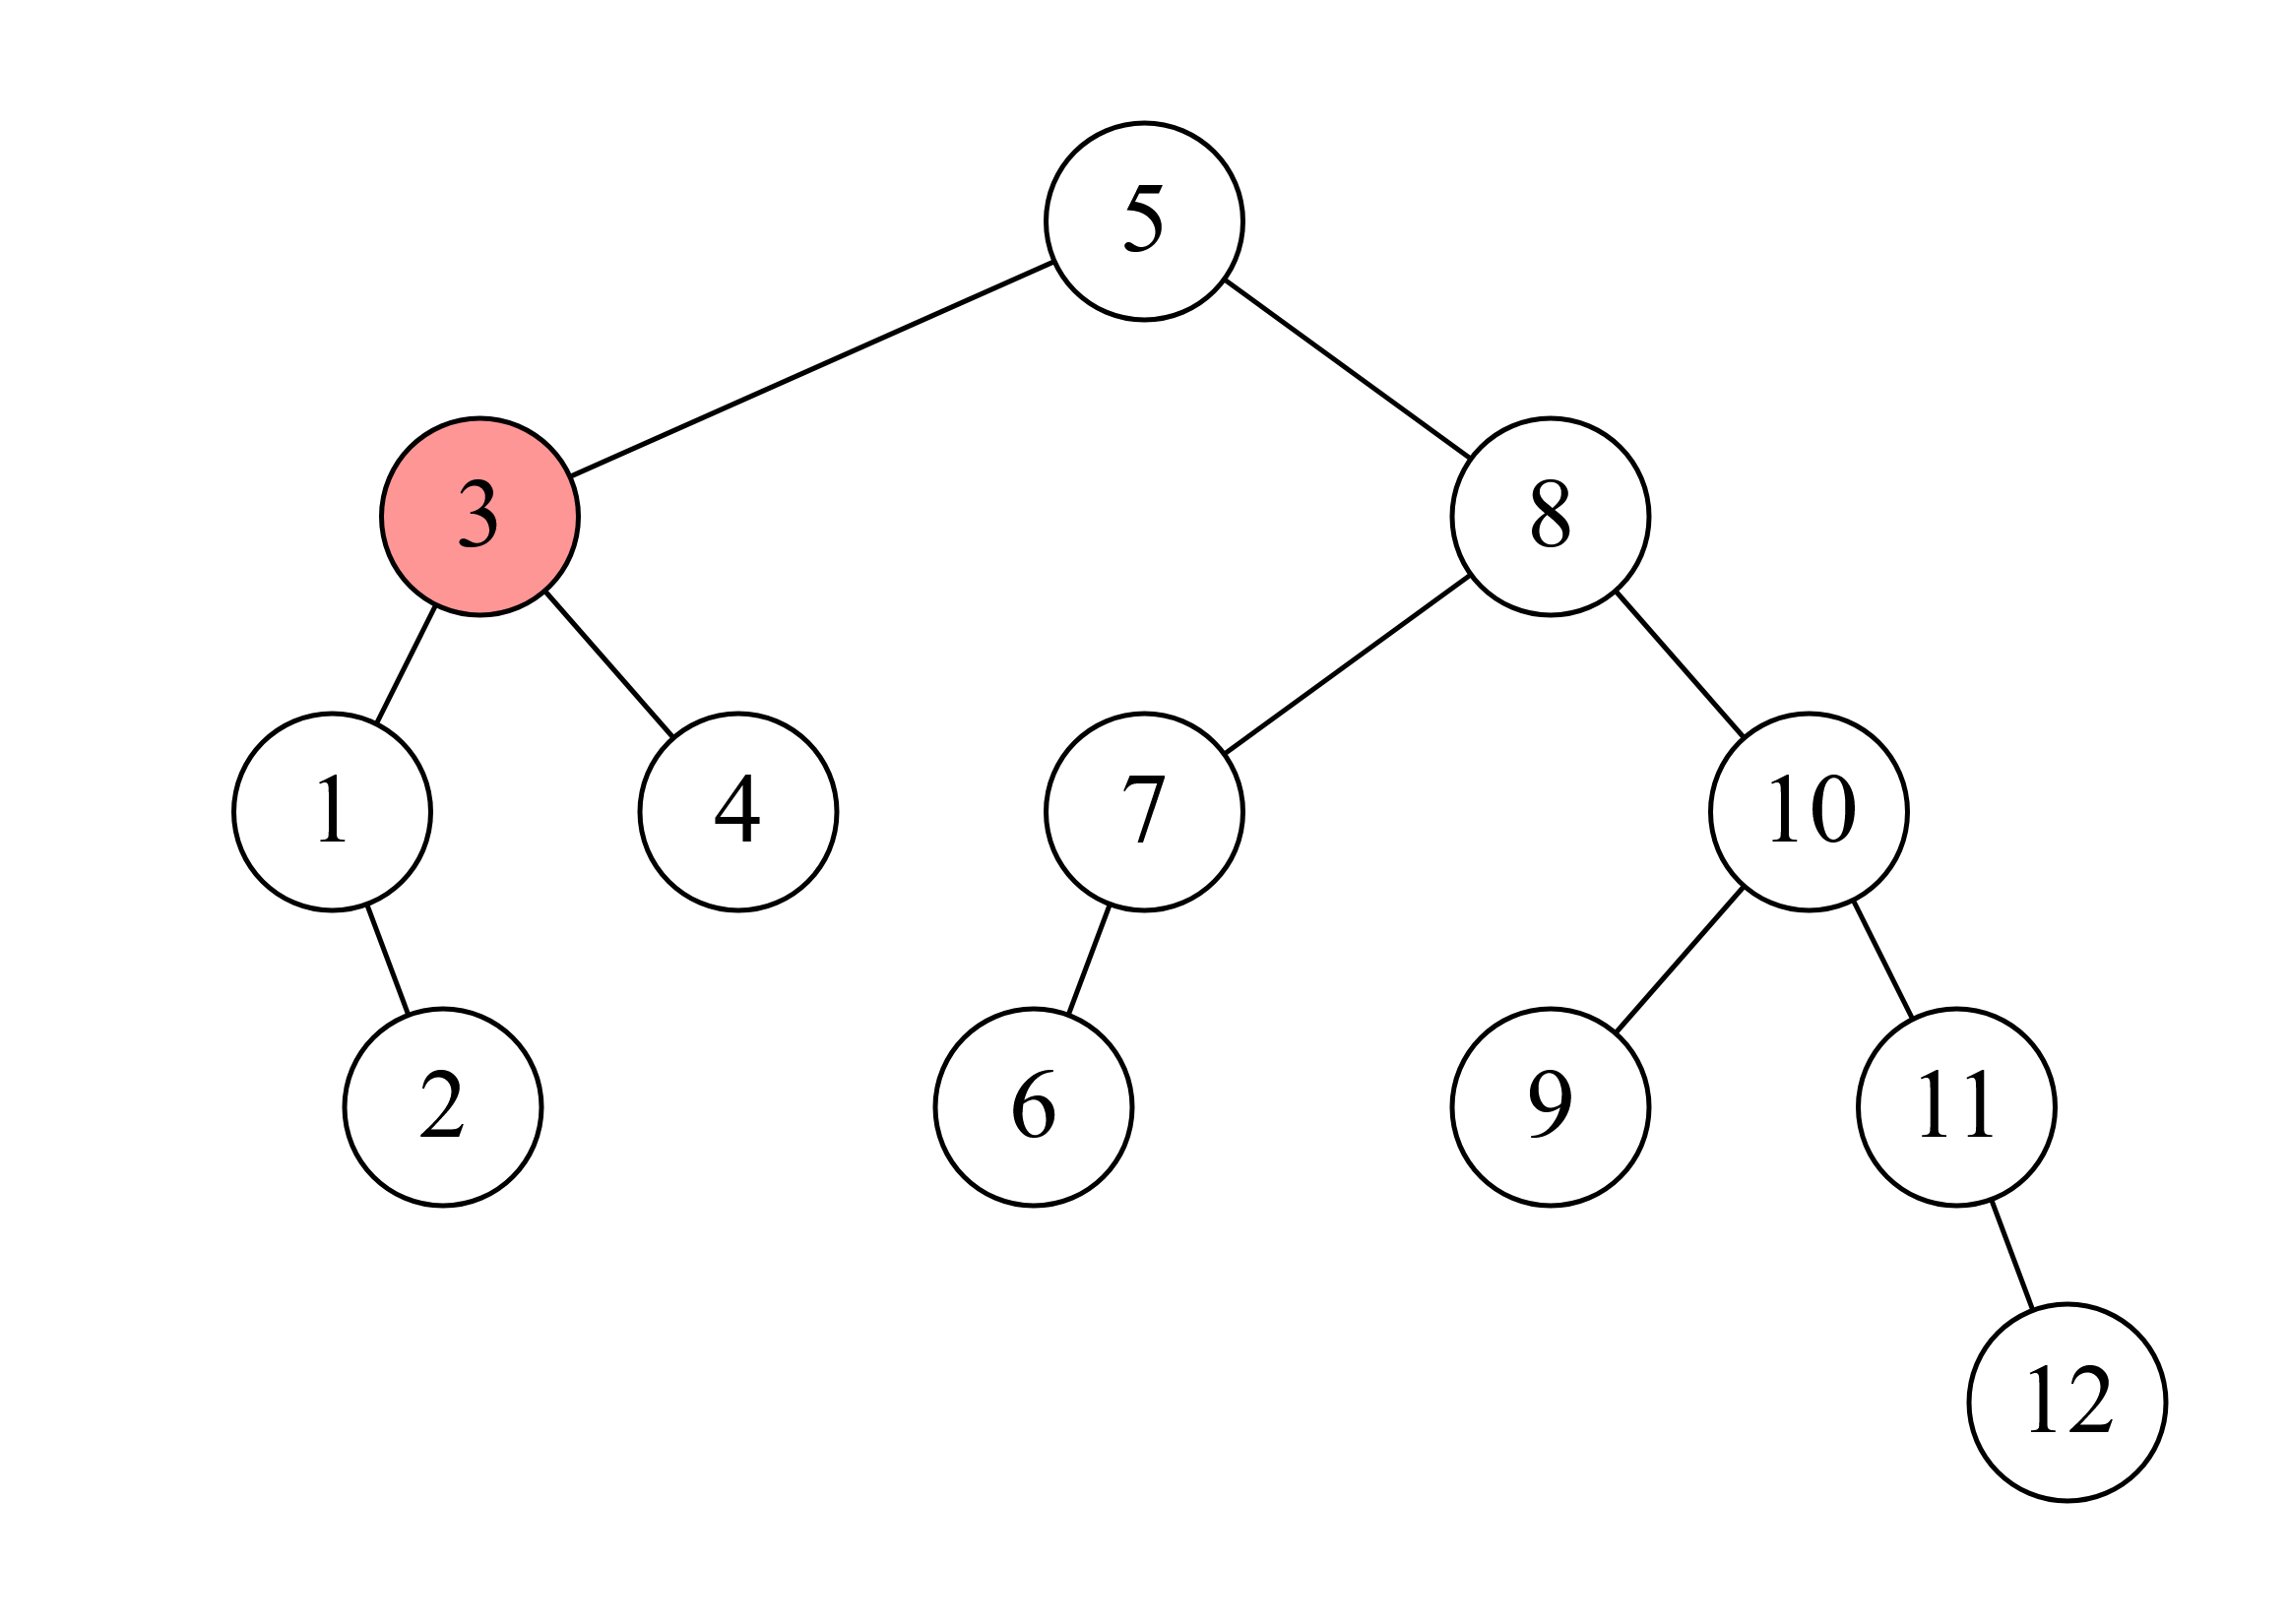
\includegraphics[width=0.42\textwidth]{img/avl.png}
        \end{figure}
        \FloatBarrier   
        \item Entfernen Sie den Wert markierten Wert aus folgendem B-Baum der Ordnung 4. Geben Sie alle Zwischenschritte an.
        \begin{figure}[h!]
            \centering
            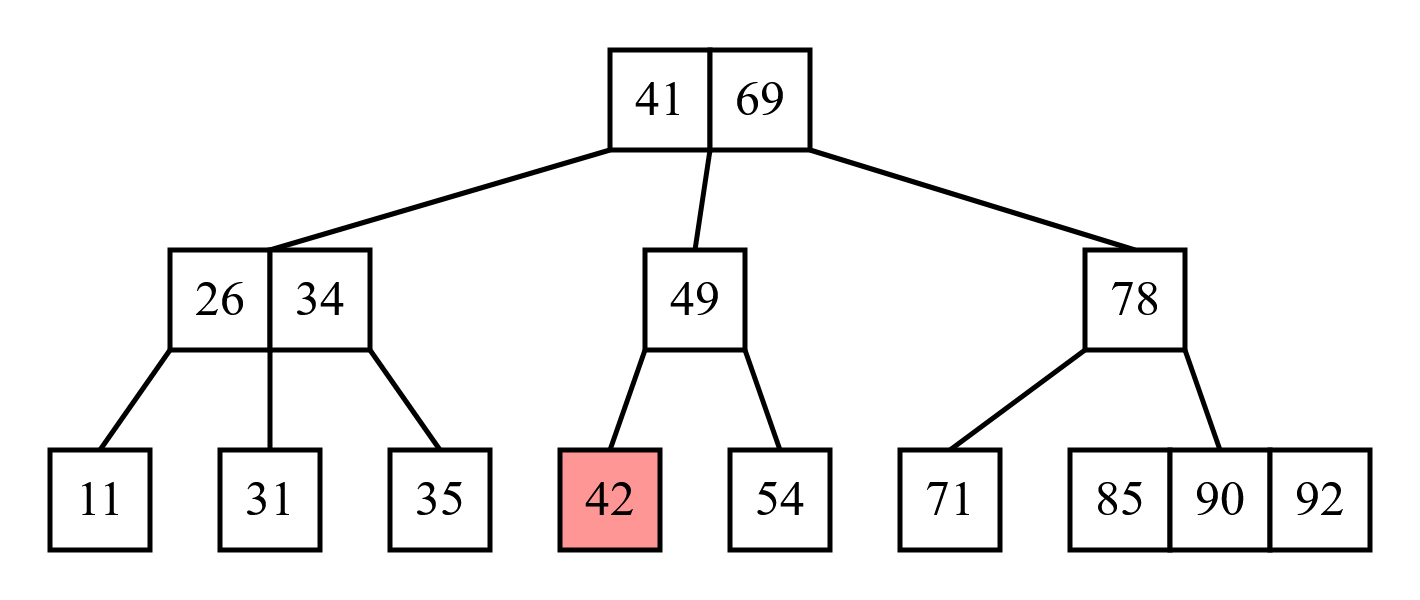
\includegraphics[width=0.5\textwidth]{img/b_tree.png}
        \end{figure}
        \FloatBarrier   
    \end{enumerate}
\end{aufgabe}
\ifcsdef{showLoesung}{}{\newpage}
\begin{aufgabe}{7}{Graphalgorithmen}
    \begin{enumerate}
        \item Demonstrieren Sie den Algorithmus zur topologischen Sortierung an folgendem Graphen:
        \begin{figure*}[h!]
            \centering
            \begin{tikzpicture}[scale=0.15]
            \tikzstyle{every node}+=[inner sep=0pt]
            \draw [black] (16.5,-18) circle (3);
            \draw (16.5,-18) node {$1$};
            \draw [black] (28.4,-18) circle (3);
            \draw (28.4,-18) node {$2$};
            \draw [black] (40.7,-18) circle (3);
            \draw (40.7,-18) node {$3$};
            \draw [black] (16.5,-29.9) circle (3);
            \draw (16.5,-29.9) node {$4$};
            \draw [black] (28.4,-29.9) circle (3);
            \draw (28.4,-29.9) node {$5$};
            \draw [black] (40.7,-29.9) circle (3);
            \draw (40.7,-29.9) node {$6$};
            \draw [black] (19.5,-18) -- (25.4,-18);
            \fill [black] (25.4,-18) -- (24.6,-17.5) -- (24.6,-18.5);
            \draw [black] (28.4,-26.9) -- (28.4,-21);
            \fill [black] (28.4,-21) -- (27.9,-21.8) -- (28.9,-21.8);
            \draw [black] (19.5,-29.9) -- (25.4,-29.9);
            \fill [black] (25.4,-29.9) -- (24.6,-29.4) -- (24.6,-30.4);
            \draw [black] (16.5,-26.9) -- (16.5,-21);
            \fill [black] (16.5,-21) -- (16,-21.8) -- (17,-21.8);
            \draw [black] (18.62,-27.78) -- (26.28,-20.12);
            \fill [black] (26.28,-20.12) -- (25.36,-20.33) -- (26.07,-21.04);
            \draw [black] (38.54,-20.09) -- (30.56,-27.81);
            \fill [black] (30.56,-27.81) -- (31.48,-27.62) -- (30.78,-26.9);
            \draw [black] (37.7,-29.9) -- (31.4,-29.9);
            \fill [black] (31.4,-29.9) -- (32.2,-30.4) -- (32.2,-29.4);
            \draw [black] (40.7,-21) -- (40.7,-26.9);
            \fill [black] (40.7,-26.9) -- (41.2,-26.1) -- (40.2,-26.1);
            \end{tikzpicture}
        \end{figure*}
        \FloatBarrier
        Wählen Sie dabei stets den Knoten mit der kleinsten Zahl zuerst, wenn Sie die Wahl haben.
        Geben Sie die topologische Sortierung an, die Sie erhalten, sowie die Reihenfolge, in der Sie die Knoten des Graphen entdecken.
        \item
        Gesucht wird ein minimaler Spannbaum in folgendem Graph:
        \begin{figure*}[h!]
            \centering
            \begin{tikzpicture}[scale=0.15]
                \tikzstyle{every node}+=[inner sep=0pt]
                \draw [black] (16.5,-18) circle (3);
                \draw (16.5,-18) node {$1$};
                \draw [black] (28.4,-18) circle (3);
                \draw (28.4,-18) node {$2$};
                \draw [black] (40.7,-18) circle (3);
                \draw (40.7,-18) node {$3$};
                \draw [black] (16.5,-29.9) circle (3);
                \draw (16.5,-29.9) node {$4$};
                \draw [black] (28.4,-29.9) circle (3);
                \draw (28.4,-29.9) node {$5$};
                \draw [black] (40.7,-29.9) circle (3);
                \draw (40.7,-29.9) node {$6$};
                \draw [black] (30.56,-27.81) -- (38.54,-20.09);
                \draw (33.53,-23.47) node [above] {$1$};
                \draw [black] (18.62,-27.78) -- (26.28,-20.12);
                \draw (21.93,-22.47) node [left] {$2$};
                \draw [black] (16.5,-21) -- (16.5,-26.9);
                \draw (16,-23.95) node [left] {$3$};
                \draw [black] (25.4,-18) -- (19.5,-18);
                \draw (22.45,-17.5) node [above] {$4$};
                \draw [black] (31.4,-18) -- (37.7,-18);
                \draw (34.55,-17.5) node [above] {$5$};
                \draw [black] (28.4,-21) -- (28.4,-26.9);
                \draw (27.9,-23.95) node [left] {$6$};
                \draw [black] (31.4,-29.9) -- (37.7,-29.9);
                \draw (34.55,-29.4) node [above] {$7$};
                \draw [black] (40.7,-21) -- (40.7,-26.9);
                \draw (40.2,-23.95) node [left] {$8$};
                \draw [black] (19.5,-29.9) -- (25.4,-29.9);
                \draw (22.45,-29.4) node [above] {$9$};
            \end{tikzpicture}
        \end{figure*}
        \FloatBarrier
        Geben Sie Reihenfolge an, in der Sie die Kanten des MST bei Anwendung des Algorithmus von Kruskal erhalten.
        Geben Sie die außerdem die Reihenfolge an, in der Sie sie beim Algorithmus von Prim erhalten.
        Die Kantengewichte genügen.
    \end{enumerate}
\end{aufgabe}

\end{document}